\apendice{Especificación de diseño}

\section{Introducción}
En este apartado se va a explicar el porqué del diseño de los datos, la arquitectura, los procesos y la interfaz gráfica de la aplicación.\\
Lo que se pretende con este apartado es que se conozca el porqué de la toma de decisiones con respectos a los aspectos arriba comentados y los motivos que han llevado a tomar esa decisión.
\section{Diseño de datos}
Los principales datos con los que se trabaja en esta aplicación son los datos bibliográficos y como ya se explicó en la memoria, concretamente en el apartado \textbf{5.4 Formato de almacenamiento}. En ese apartado se explica que se presentaron 3 formatos alternativos para el manejo de los datos y que finalmente se acabó eligiendo el formato \emph{BibTeX} por sus etiquetas más descriptivas y su mayor facilidad de trabajo, ya que existen un gran número librerías que permiten un fácil manejo de los datos.
\section{Diseño procedimental} \label{diseño procedimental}
\begin{figure}[H]
	\centering
	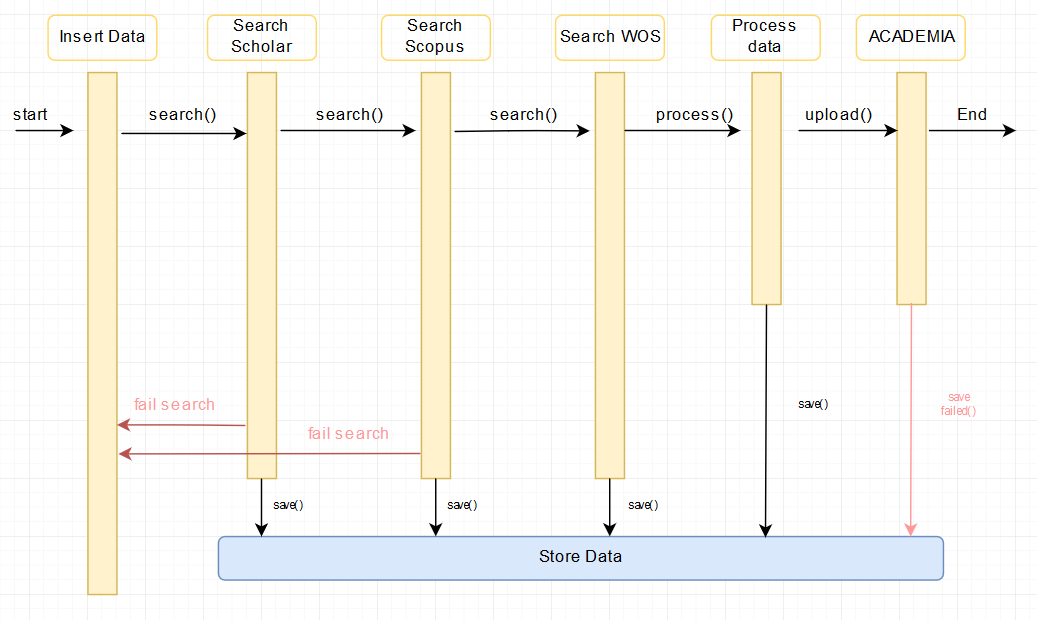
\includegraphics[width=1\textwidth]{procedimental}
	\caption{Diagrama de secuencia de la aplicación.}
	\label{fig:procedmiental}
\end{figure}

Como podemos ver en la figura \ref{fig:procedmiental} se trata de un modelo secuencial y con una sola dirección , esto se debe a que la idea que se concibió para esta aplicación es como un herramienta sencilla de fácil usabilidad pero que fuera perfectamente funcional. A continuación se va a explicar el proceso que se ve en la imagen:
\begin{enumerate}
	\item Introduce los datos referentes a la búsqueda.
	\item Se procede a la extracción de los datos en \emph{Google Scholar}, si la extracción no diera resultados el usuario sería preguntado para introducir los datos de nuevo.
	\item Se procede a la extracción de los datos en \emph{Scopus} si la extracción no diera resultados el usuario sería preguntado para introducir los datos de nuevo.
	\item Se procede a la extracción de los datos en \emph{Web of Science}
	\item Se procesan los datos
	\item Se accede a ACADEMIA y se procede a la subida de los datos resultantes del anterior paso.
	\item Los datos que no han podido ser subidos son almacenados para una posterior revisión por parte del usuario.
\end{enumerate}

\section{Diseño arquitectónico}
\subsection{Modelo-Vista-Controlador}

El Modelo-vista-controlador es un patrón de arquitectura de software, que se basa en la separación de los datos y la funcionalidad de la representación gráfica, para ello se sirve de tres componentes: modelo, vista, controlador. Lo que se persigue con este modelo es la separación de conceptos y la reutilización de código.
\begin{figure}[H]
	\centering
	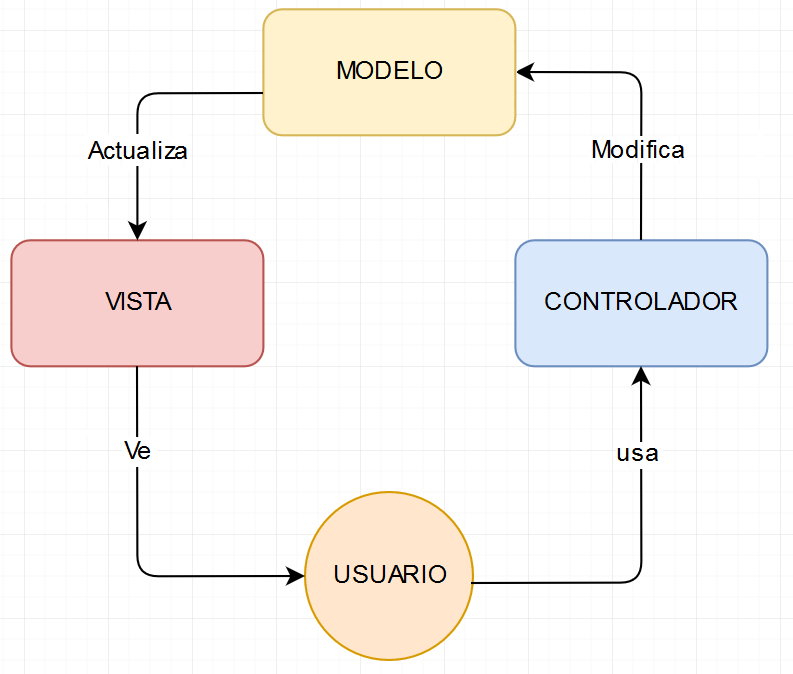
\includegraphics[width=1\textwidth]{MVC}
	\caption{Diagrama de MVC.}
	\label{fig:MVC}
\end{figure}
\begin{itemize}
	\item \textbf{Modelo.} Es la representación de la información con la cual la aplicación realiza las operaciones, es decir gestiona todos los accesos del sistema a la información. Envía a la vista la información necesaria en cada momento y que es solicitada por parte del usuario a través del controlador.
	\item \textbf{Vista.} Muestra el \emph{modelo} es decir la información, en un formato adecuado para que sea entendida por el usuario y que le permita interactuar de una manera simple y adecuada.
	\item \textbf{Controlador.} El controlador responde a los eventos fruto de la interacción del usuario con la \emph{vista} y envía peticiones al \emph{modelo} para actualizar la información en la \emph{vista}. Podemos decir que el controlador hace de intermediario entre el \emph{modelo} y la \emph{vista}
\end{itemize}

Como vemos en la figura \ref{fig:MVC}:
\begin{enumerate}
	\item El usuario interactúa con la vista.
	\item El controlador recibe una petición de acción.
	\item El controlador realiza las peticiones para la modificación del modelo.
	\item El modelo envía la nueva información a mostrar a la vista.
	\item La vista se encarga de mostrar la información de la manera adecuada.
	\item El usuario ve la nueva información y empieza de nuevo el proceso.
\end{enumerate}
\subsection{Arquitectura General}
La arquitectura general de la aplicación vista de una forma simplificada sería:
\begin{figure}[H]
	\centering
	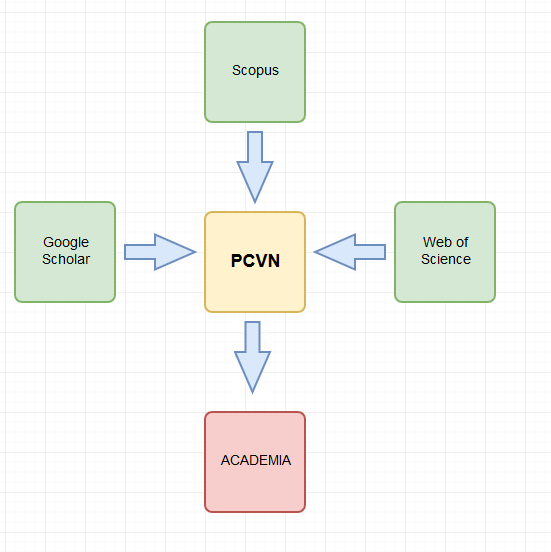
\includegraphics[width=0.8\textwidth]{esquema}
	\caption{Arquitectura de la aplicación.}
	\label{fig:esquema}
\end{figure}
Como vemos en la sección \ref{fig:esquema} se efectúa todo el proceso de manera secuencial, se extraen los datos , se procesan y modelan adecuadamente y finalmente se suben a ACADEMIA como se ha explicado en \ref{diseño procedimental}
\section{Diseño de interfaces}
Para el diseño de la interfaz se buscaba sencillez y funcionalidad, dos requisitos que se han solventado con el uso de la librería para \emph{Python} \emph{Tkinter}, la cual ofrece funcionalidades más que suficientes y un uso sencillo y eficaz.

Con el fin de mejorar la experiencia del usuario con el uso de la interfaz se han integrado una serie de contenedores de texto y barras de progreso que: 
\begin{itemize}
	\item Informan al usuario de la tarea que se está llevando a cabo y de qué es lo que pasará después.
	\item Informa al usuario del progreso de la tarea y cuánto falta para la finalización de esta.
\end{itemize}

A continuación vamos a ver unas imágenes de ejemplo de cómo se ve esta interfaz.
\begin{figure}[H]
	\centering
	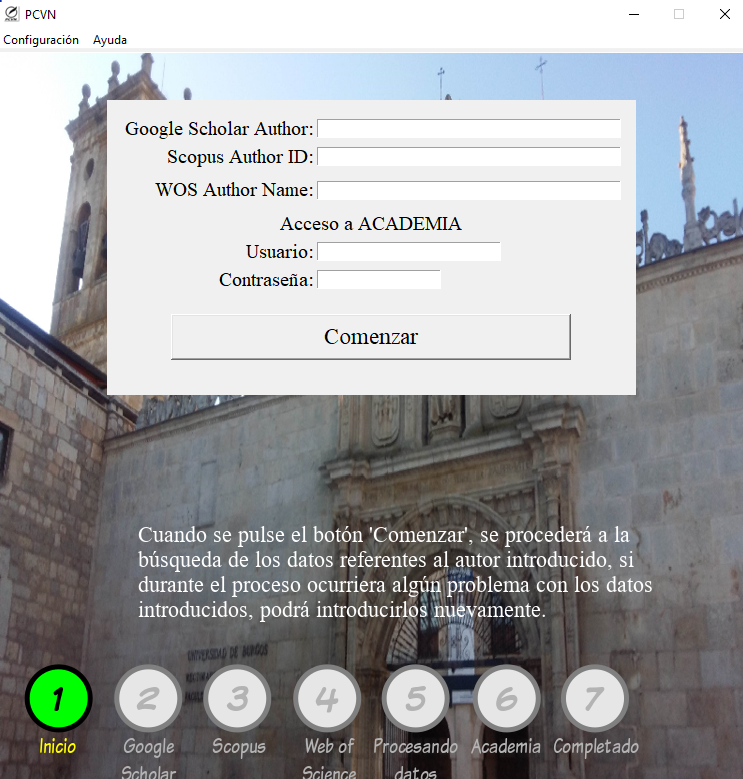
\includegraphics[width=1\textwidth]{GUI1}
	\caption{Imagen de ejemplo de la interfaz gráfica.}
	\label{fig:gui1}
\end{figure}
Vemos en la figura \ref{fig:gui1} una interfaz simple y sencilla, sin objetos agresivos o intrusivos.
\begin{figure}[H]
	\centering
	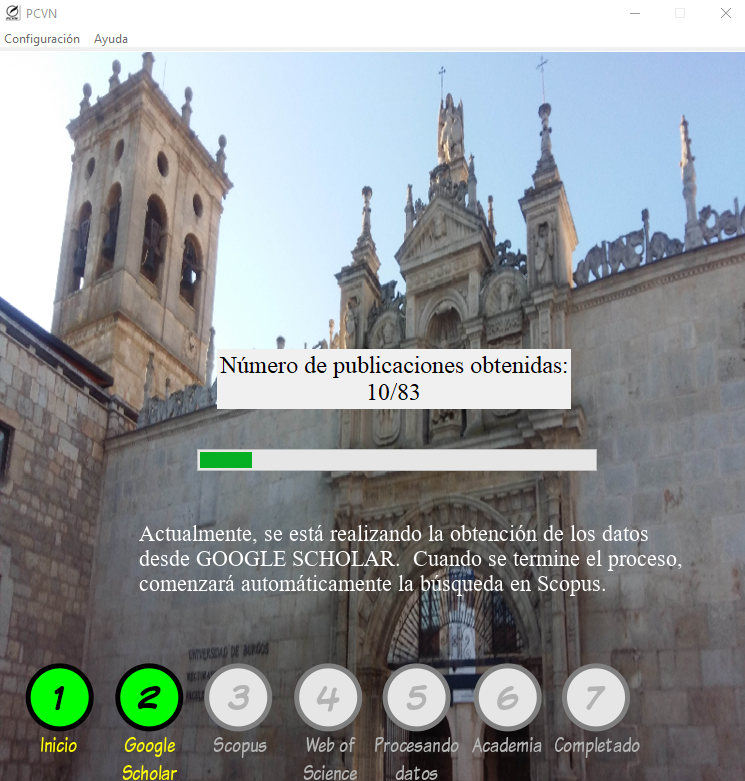
\includegraphics[width=1\textwidth]{GUI2}
	\caption{Imagen de ejemplo de la interfaz gráfica.}
	\label{fig:gui2}
\end{figure}

Vemos en la figura \ref{fig:gui2} como en todo momento el usuario es informado de lo que está pasando y del estado de la tarea.

Se ha utilizado una gama de colores suaves y un fondo sobrio y elegante para conservar el corte simplista y estético de la aplicación que hace que los textos importantes sea lo que más llame la atención al usuario.

El único momento en el que se han utilizado colores fuertes y llamativos es cuando el usuario introduce erróneamente los datos, esto es para informar al usuario de que es lo que debe corregir como vemos en la figura \ref{fig:gui4} 
\begin{figure}[H]
	\centering
	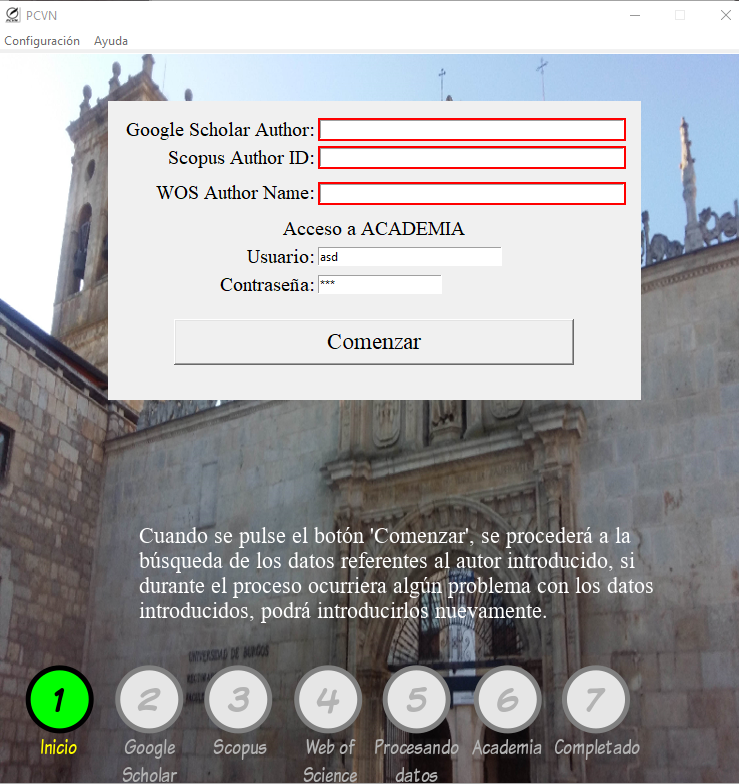
\includegraphics[width=1\textwidth]{GUI4}
	\caption{Imagen de ejemplo de error en la interfaz gráfica.}
	\label{fig:gui4}
\end{figure}

Para informar al usuario de errores acontecidos durante la normal ejecución de la aplicación se han utilizado ventanas emergentes que captan la atención del usuario y lo hacen centrarse en el mensaje que este transmite como se puede ver en la  figura \ref{fig:gui3}
\begin{figure}[H]
	\centering
	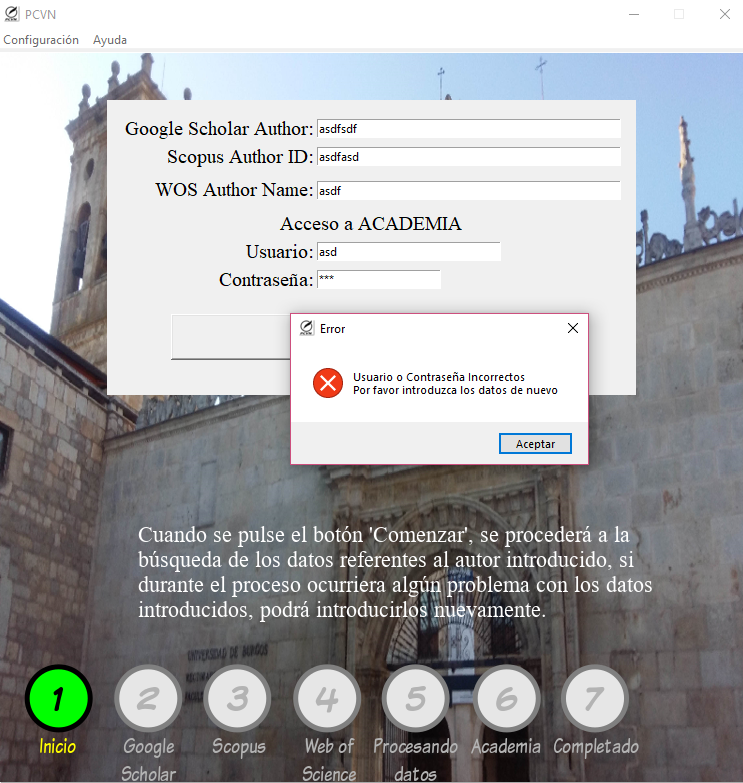
\includegraphics[width=1\textwidth]{GUI3}
	\caption{Imagen de ejemplo de ventana emergente.}
	\label{fig:gui3}
\end{figure}
